\providecommand{\main}{..}
\documentclass[main.tex]{subfiles}

\begin{document}
\chapter{Acoustic Design}
In this chapter all aspects related to the acoustic and physical design of the speakers will be discussed.
\section{Cabinet Design}
\subsection{Driver Choice}
An important defining step in the early stage of speaker design is the choice of speaker drivers. 
This determines the type of speaker, the quality of the speaker, the size of the speaker, and the cost of the speaker.
Because of this careful consideration must be taken to make sure the selected drivers suit the specific application and are good enough quality.

The drivers chosen were the ...

The woofer was chosen as it was suitable for a sealed cabinet design, and gives a cabinet size in the range that we desire.
The specific discussion of why this driver is suitable is in \ref{woofercalcs}.
The tweeter was chosen as its frequency range crosses over significantly with that of the woofers, ensuring that the speaker will have good performance over the full output frequency range.
The frequency responses can be seen in figure \ref{fig:driverFreqResponse}.
\begin{figure}
    \centering
    Frequency responses of the drivers
    \caption{The frequency responses of the two selected drivers}
    \label{fig:driverFreqResponse}
\end{figure}

\subsection{Woofer Calculations}
\label{woofercalcs}
Tweeters are totally enclosed devices and as such they can simply be mounted with no consideration having to be given to how or what is it is mounted on.
Woofers alternatively pose a greater complication as their performance is heavily determined by the physical enclosure it is mounted on.

The two main types of enclosure are sealed and ported enclosures.
Ported enclosures give better lower frequency response, but also results in higher volume cabinets for the same driver.
In addition, ported cabinets require much more precise construction and tuning, as the resonant frequency of the enclosure is extremely important to the performance.
While ported cabinets require precise tuning, the only important attribute of a sealed cabinet is its volume, which affects the actual system $Q_{tc}$.
This is a design choice, which is commonly chosen to be equal to $0.707$ in order to give maximal flatness.
A higher value of $Q_{tc}$ results in a peak resonance, while lower $Q_{tc}$ gives a steeper frequency roll off.
This can be seen in figure \ref{fig:qtcplot}.
In order to obtain a flat frequency roll off a value of 0.707 was used in this design.
\begin{figure}
    \centering
    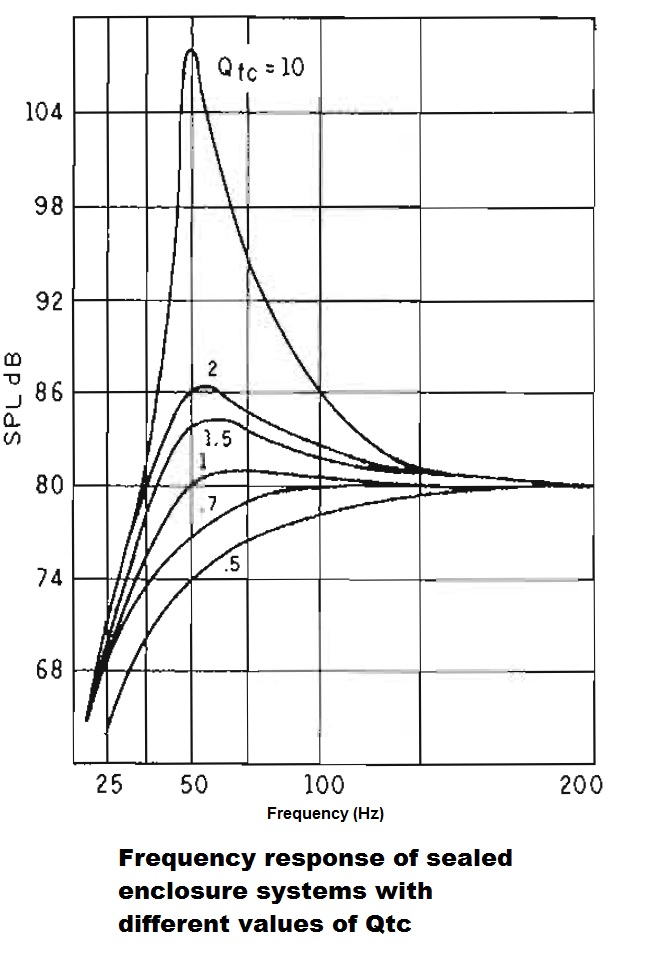
\includegraphics[width=0.5\textwidth]{figs/qtcResponsePlot.jpg}
    \caption{}
    \label{fig:qtcplot}
\end{figure}

Using the Thiele/Small\footnote{Thiele/Small parameters of speaker drivers are the parameters that } parameters from the data sheet of the woofer, the specific parameters of the selected driver can be calculated.

The first parameter to consider is the efficiency bandwidth product (EBP).
This determines whether the driver is suited for a sealed or ported enclosure, and is found to be:
\begin{equation}
    \mbox{EBP} = \frac{f_s}{Q_{es}} = ??
\end{equation}
where $f_s$ is the resonant frequency of the driver and $Q_{es}$ is the electrical Q of the driver at $f_s$.
This value shows that is suitable for mounting in a sealed enclosure.

The internal volume of the enclosure can then be calculated using:
\begin{equation}
    V_b = \frac{V_{as}}{\left(\frac{Q_{tc}}{Q_{ts}}\right)^2-1}=?
\end{equation}
where $Q_{tc}=0.707$ as decided earlier, $V_{as}$ is the air volume equal to the compliance of the driver suspension and $Q_{ts}$ is the total system $Q$ at $f_s$.
These are obtained from the datasheet for the driver.

The frequency where the power dropped by the system is 3dB can also be found, which gives an indication of the lower frequency range of the total speaker:
\begin{equation}
    f_3 = \frac{Q_{tc}f_s}{Q_{ts}}\sqrt{\frac{\frac{1}{Q_{tc}^2}-2+\sqrt{\left(\frac{1}{Q_{tc}^2}-2\right)^2+4}}{2}}=?
\end{equation}
\subsection{Dimensions}
Now that the internal volume of the enclosure has been calculated, the dimensions of the speaker can now be decided.
In order to 
Aspect ratio $1/phi:1:phi$ to prevent standing waves.
11mm mdf significant enough to reinforce
\section{Construction and Manufacturing}
\section{Testing}
\subsection{Overview}
\subsection{Results}

\end{document}